\documentclass[a4paper]{scrartcl}
\usepackage[finnish]{babel}
\usepackage[utf8]{inputenc}
\usepackage[T1]{fontenc}
\usepackage{mathptmx}
\usepackage[numbers]{natbib}
\usepackage{hyperref}
\usepackage{tikz-uml}
\usepackage{enumitem}
\usepackage{calc}
\usepackage{graphicx}
\setlist[description]{font={\rmfamily}}
\addtokomafont{disposition}{\rmfamily}

\subject{Aineopintojen harjoitustyö: Tietokantasovellus}
\author{Jarno Leppänen}
\title{Divvd -- Useilla valuutoilla toimiva kustannusten jako}
\subtitle{Dokumentaatio}
\date{23.3.2014}

\begin{document}

\maketitle

\section{Johdanto}

Kustannusten jako on tavallinen ongelma illanvietoissa ystävien
kanssa tai taloudenpidossa puolison tai kämppäkavereiden välillä. Erityisen
hankalaksi tehtävä osoittautuu, jos jaettavissa kustannuksissa on käytetty
useita eri valuuttoja. Ulkomailla matkaillessa syntyy helposti tilanteita,
joissa esimerkiksi matkaliput ja majoitukset on maksettu kotimaan valuutassaa,
mutta juoksevat kulut hoidetaan kohdemaan valuutassa. Miten kustannukset
pitäisi silloin jakaa?

Työssä toteutetaan kustannusten jakoon tarkoitettu kirjanpitojärjestelmä, jossa
kirjauksia voi tehdä eri valuutoilla. Käyttäjä voi rekisteröitymisen ja
kirjautumisen jälkeen luoda \textit{tilikirjoja}, jotka ovat kokoelmia
käyttäjän syöttämistä \textit{tilitapahtumista}. Tilitapahtumaan kirjataan
tapahtuman osapuolet sekä näiden tulot ja menot tapahtumaan liittyen.
Järjestelmä laskee tilikirjassa olevien osapuolten kokonaissaldot haluttuun
valuuttaan muunnettuna ja osaa lisäksi ehdottaa tapoja velkojen
takaisinmaksuun. Takaisinmaksujärjestely voidaan ratkaista esimerkiksi
minimoimalla järjestelyssä tapahtuvien transaktioiden
lukumäärä\cite{verhoeff2004settling}.

\subsection{Toimintaympäristö}

Ohjelma toteutetaan web-sovelluksena heroku-PaaS-palvelun päälle.
Sovelluskehyksenä käytetään herokun tukemaa node.js-ympäristöä.
Selainkäyttöliittymän sovelluskehyksenä käytetään AngularJS-kirjastoa.
Ohjelmointikielenä sekä selain-, että palvelinympäristöissä on Javascript.

Tietokantana toimii herokun tarjoama PostgreSQL. Tietokantaa käsitellään
suoraan Postgre\-SQL:n laajennetun SQL-kielen avulla. Toteutuksessa tullaan
hyödyntämään SQL-standardiin kuulumattomia trigger- ja view-mekanismeja, joten
tietokantamoduli tulee olemaan sidottu Post\-gre\-SQL-jär\-jes\-tel\-mään.

\section{Yleiskuva järjestelmästä}

\subsection{Käyttötapauskaavio}

\newcommand{\coldist}{5}
\begin{tikzpicture}
\begin{umlsystem}[x=5,fill=yellow!20]{Divvd-järjestelmä}
  \umlusecase[name=register]{rekisteröityminen}
  \umlusecase[y=-2,name=login]{kirjautuminen}
  \umlusecase[y=-4,name=ledger,width=1.5cm]{tilikirjojen käsittely}
  \umlusecase[y=-6,name=transaction,width=2.2cm]{tilitapahtumien käsittely}
  \umlusecase[y=-10,name=totals,width=2cm]{loppusaldojen tulostus}
  \umlusecase[y=-12,name=settle,width=2.9cm]{maksusuunnitelman tulostus}
  \umlusecase[y=-8,name=currency,width=2.4cm]{valuuttakurssien muokkaus}
  \umlusecase[y=-4,x=\coldist,name=add-ledger,width=1.5cm]{tilikirjan lisäys}
  \umlusecase[y=-2,x=\coldist,name=delete-ledger,width=1.5cm]{tilikirjan poisto}
  \umlusecase[y=-6,x=\coldist,name=add-transaction,width=2.2cm]{tilitapahtuman
    lisäys}
  \umlusecase[y=-10,x=\coldist,name=delete-transaction,width=2.2cm]{tilitapahtuman
    poisto}
  \umlusecase[y=-8,x=\coldist,name=edit-transaction,width=2.2cm]{tilitapahtuman
    muokkaus}
\end{umlsystem}
\umlactor[y=-6,x=-1,name=user]{käyttäjä}
\umlassoc{user}{register}
\umlassoc{user}{login}
\umlassoc{user}{ledger}
\umlassoc{user}{transaction}
\umlassoc{user}{totals}
\umlassoc{user}{settle}
\umlassoc{user}{currency}
\umlinherit{add-ledger}{ledger}
  \umlinherit{delete-ledger}{ledger}
\umlinherit{add-transaction}{transaction}
\umlinherit{delete-transaction}{transaction}
\umlinherit{edit-transaction}{transaction}
\umlinclude{ledger}{login}
\umlinclude{transaction}{add-ledger}
\end{tikzpicture}

\subsection{Käyttäjäryhmät}

\begin{description}
  \item[käyttäjä] järjestelmään rekisteröitynyt käyttäjä
\end{description}

\subsection{Käyttötapauskuvaukset}

\begin{description}[style=nextline]
  \item[tilikirjojen käsittely]{
      Kirjautunut käyttäjä voi lisätä ja poistaa tilikirjoja. Kun tilikirjan
      poistaa, kaikki siihen liittyvät tilitapahtumat, osapuolet ja valuutat
      poistuvat samalla.
    }
  \item[tilitapahtumien käsittely]{
      Kirjautunut käyttäjä voi lisätä, poistaa ja muokata tietyn tilikirjan
      tilitapahtumia. Tilitapahtumaan liittyy osapuolia sekä näiden
      tilitapatumaan liittyviä menoja ja tuloja. Menoja ja tuloja voidaan
      kirjata eri valuutoilla ja tilitapahtumien kokonaissummaa voidaan
      tarkastella haluttuun valuuttaan muunnettuna.
    }
  \item[valuuttakurssien muokkaus]{
      Kirjautunut käyttäjä voi muokata tilikirjassa olevien valuuttojen
      kursseja.
    }
  \item[loppusaldojen tulostus]{
      Kirjautunut käyttäjä voi tulostaa tilikirjan loppusaldot kaikki
      osapuolten osalta.
    }
  \item[maksusuunnitelman tulostus]{
      Kirjautunut käyttäjä pyytää järjestelmältä ehdotusta velkojen
      takaisinmaksujärjestelystä.
    }
\end{description}

\section{Järjestelmän tietosisältö}

\subsection{Käsitekaavio}

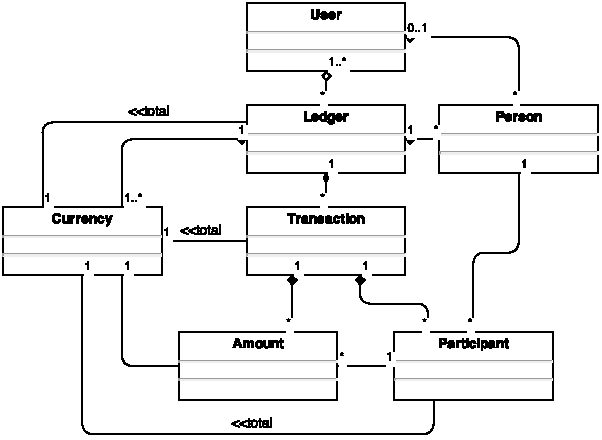
\includegraphics[scale=1.4]{db}

\subsection{Tietokohteet}

\subsubsection{User}
\begin{tabular}{ | l | l | l | }
  \hline
  \textbf{Attribuutti} & \textbf{Arvojoukko} & \textbf{Kuvailu} \\ \hline
  Name & Merkkijono & Käyttäjän nimi \\ \hline
  Hash & 256-bittinen binäärinen merkkijono &
    Salasanasta laskettu hajautusarvo
    \\ \hline
  Salt & 64-bittinen binäärinen merkkijono & Satunnainen binäärinen merkkijono
    \\ \hline
\end{tabular}

\subsubsection{Ledger}
\begin{tabular}{ | l | l | l | }
  \hline
  \textbf{Attribuutti} & \textbf{Arvojoukko} & \textbf{Kuvailu} \\ \hline
  Title & Merkkijono & Tilikirjan nimi \\ \hline
\end{tabular}

\subsubsection{Currency}
\begin{tabular}{ | l | l | l | }
  \hline
  \textbf{Attribuutti} & \textbf{Arvojoukko} & \textbf{Kuvailu} \\ \hline
  Code & Merkkijono & Valuutan nimi tai lyhenne \\ \hline
  Rate & Desimaaliluku & Valuutan kurssi \\ \hline
\end{tabular}

\subsubsection{Transaction}
\begin{tabular}{ | l | l | l | }
  \hline
  \textbf{Attribuutti} & \textbf{Arvojoukko} & \textbf{Kuvailu} \\ \hline
  Date & Päivämäärä & Tilitapahtuman päivämäärä \\ \hline
  Description & Merkkijono & Selite \\ \hline
  Location & Merkkijono & Tilitapahtuman paikka \\ \hline
  Type & Merkkijono & Tilitapahtuman tyyppi \\ \hline
  Transfer & Totuusarvo & Totuusarvo, joka kertoo, onko tilitapahtuma
    rahansiirto vai kulu \\ \hline
\end{tabular}

\subsubsection{Participant}
\begin{tabular}{ | l | l | l | }
  \hline
  \textbf{Attribuutti} & \textbf{Arvojoukko} & \textbf{Kuvailu} \\ \hline
  ShareDebt & Totuusarvo & Tosi, jos osapuoli osallistuu
kattamattomiin kuluihin \\ \hline
\end{tabular}

\subsubsection{Person}
\begin{tabular}{ | l | l | l | }
  \hline
  \textbf{Attribuutti} & \textbf{Arvojoukko} & \textbf{Kuvailu} \\ \hline
  Name & Merkkijono & Osapuolen nimi \\ \hline
\end{tabular}

\subsubsection{Amount}
\begin{tabular}{ | l | l | l | }
  \hline
  \textbf{Attribuutti} & \textbf{Arvojoukko} & \textbf{Kuvailu} \\ \hline
  Amount & Desimaaliluku & Rahamäärä \\ \hline
\end{tabular}

\section{Relaatiotietokantakaavio}

Jokaisella tietokannan taululla on tyyppiä SERIAL oleva synteettinen
primäärinen avain nimellä \textit{taulu}\_id. Näitä avaimia ei ole piirretty
kaavioon.

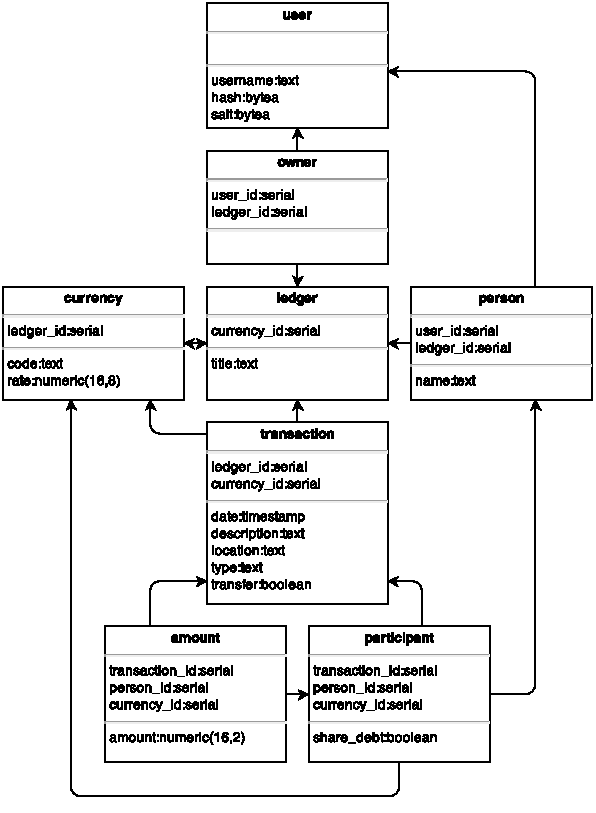
\includegraphics[scale=1.35]{schema}

\section{Käyttöliittymä}

Web-käyttöliittymä toteutetaan "single page"-applikaationa, jossa selaimen
lataama javascript-käyttöliittymä keskustelee palvelimen JSON-rajapinnan
kanssa ja päivittää selaimen osoitekenttää kulloinkin näytettävää resurssia
vastaavaksi. Arkkitehtuurin ansiosta yksittäinen käyttöliittymänäkymä voi
päivittää tietokantaa osissa ilman, että näkymää tarvitsee ladata palvelimelta
uudelleen.

\subsection{Käyttöliittymäkaavio}

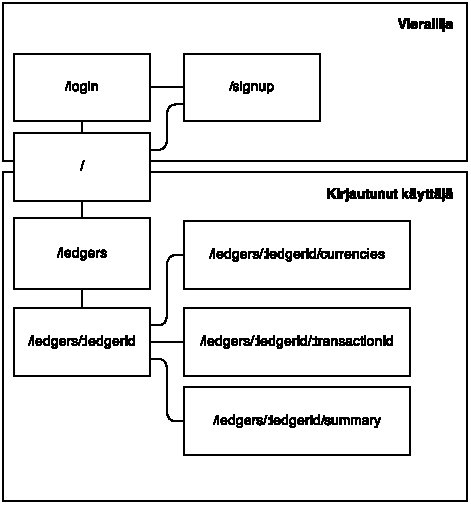
\includegraphics[scale=1.5]{ui}

\subsection{Näkymät}

\begin{description}[style=nextline]
  \item[/]{
      Etusivu näyttää kirjautumattomalle vierailijalle kirjautumislomakkeen sekä
      linkin rekisteröitymissivulle. Kirjautunut käyttäjä näkee listan omista
      tilikirjoistaan.
    }
  \item[/login]{
      Kirjautumissivu, joka näyttää pelkän lomakkeen. Onnistuneen kirjautumisen
      jälkeen käyttäjä ohjataan kirjautuneena etusivulle.
    }
  \item[/signup]{
      Rekistereöitymissivu. Onnistuneen rekisteröinnin jälkeen käyttäjä ohjataan
      kirjautuneena etusivulle.
    }
  \item[/ledgers]{
      Tilikirjojen listaussivu näyttää rekisteröityneen käyttäjän tilikirjat.
      Listaussivun kautta tilikirjoja voi lisätä tai poistaa. Sivulta voi myös
      siirtyä tarkastelemaan yksittäisen tilikirjan tilitapahtumia.
    }
  \item[/ledgers/:ledgerId]{
      Tilikirjan tilitapahtumien listaussivu näyttää kaikki tilikirjaan
      liittyvät tilitapahtumat. Sivu voidaan näyttää vain, jos kirjautunut
      käyttää omistaa tilikirjan. Sivun avulla tilitapahtumia voi lisätä ja
      poistaa. Sivun kautta pääsee myös muokkaamaan yksittäistä tilitapahtumaa.
    }
  \item[/ledgers/:ledgerId/summary]{
      Tilikirjan yhteenveto listaa kaikkien tilikirjaan liittyvien osapuolten
      kokonaissaldot sekä järjestelmän automaattisesti tuottaman
      velanmaksusuunnitelman, jonka voi halutessaan siirtää tilitapahtumaksi,
      jolloin tilikirjan saldot tasapainottuvat.
    }
  \item[/ledgers/:ledgerId/currencies]{
      Valuuttojen muokkaussivu näyttää tilikirjaan liittyvät valuutat
      kursseineen.  Sivun avulla valuuttoja voi lisätä, poistaa ja muokata.
    }
  \item[/ledgers/:ledgersId/:transactionId]{
      Tilitapahtumasivulla tilitapahtumaa voi muokata. Tilitapahtumaan voi
      lisätä osapuolten tekemiä maksuja ja velkasitoumuksia.
    }
\end{description}

\section{JSON-rajapinta}

Web-käyttöliittymä keskustelee tietokannan kanssa palvelimen tarjoaman
JSON-rajapinnan kautta. Rajapinnan avulla järjestelmän laajentaminen muille
alustoille on yksinkertaista. JSON-rajapinta on julkinen, joten myös kolmannet
osapuolet voivat halutessaan hyödyntää sitä.

\subsection{Tunnistautuminen}

Rajapinta vaatii tunnistautumista joko HTTP Basic -autentikoinnin tai
selainevästeiden avulla. Selaimen uloskirjautumisen mahdollistamiseksi
kirjautumiseen liittyvät osoitteet /api/login,
/api/logout, /api/signup ja /api/account eivät kuitenkaan hyväksy
HTTP Basic -autentikointia.

Rajapinta vastaa tunnistautumattomaan pyyntöön statuskoodilla 400.
Vastauksen WWW-Authenticate -otsakkeen voi halutessaan muuttaa
Custom-tyyppiseksi liittämällä palvelupyyntöön GET-parametri auth=hidden.
Näin voidaan estää selaimen automaattisesti näyttämä kirjautumisikkuna.

\subsection{Palveluosoitteet}

JSON-rajapinta on vielä keskeneräinen. Toteutetut osoitteet on dokumentoitu
toiminnallisuuden oheiseen listaan. Parametreja ja paluuviestejä ei kuitenkaan
ole vielä dokumentoitu.

\begin{description}[style=nextline]
  \item[POST /api/login]{
      Kirjaa käyttäjän sisään.
    }
  \item[POST /api/signup]{
      Rekisteröi käyttäjän.
    }
  \item[GET /api/account]{
      Palauttaa kirjautuneen käyttäjän tiedot.
    }
  \item[GET /api/logout]{
      Kirjaa ulos käyttäjän.
    }

  \item[GET /api/users]{
      Palauttaa listan käyttäjistä. Hyväksyy myös HTTP Basic -autentikoinnin.
    }
  \item[GET /api/users/:userName]{
      Palauttaa käyttäjän. Hyväksyy myös HTTP Basic -autentikoinnin.
    }
  \item[GET /api/users/:userName/ledgers]{
    }

  \item[POST /api/ledgers]{
    }
  \item[GET /api/ledgers/:ledgerId]{
    }
  \item[PUT /api/ledgers/:ledgerId]{
    }
  \item[DELETE /api/ledgers/:ledgerId]{
    }
  \item[GET /api/ledgers/:ledgerId/currencies]{
    }
  \item[PUT /api/ledgers/:ledgerId/currencies]{
    }
  \item[GET /api/ledgers/:ledgerId/transactions]{
    }
  \item[PUT /api/ledgers/:ledgerId/transactions]{
    }

  \item[GET /api/transactions/:transactionId]{
    }
  \item[PUT /api/transactions/:transactionId]{
    }
  \item[DELETE /api/transactions/:transactionId]{
    }

  \item[GET /api/currencies/:currencyId]{
    }
  \item[PUT /api/currencies/:currencyId]{
    }
  \item[DELETE /api/currencies/:currencyId]{
    }
\end{description}

\bibliographystyle{plainnat}
\bibliography{dokumentaatio}
\end{document}
